\documentclass[aspectratio=169, 10pt]{beamer}
\usepackage{graphicx} % Required for inserting images
\usepackage{booktabs}
\usepackage{adjustbox}
\usepackage[utf8]{inputenc}
\usepackage{lmodern}
\usepackage{tcolorbox}
\usetheme{Boadilla}
%\usefonttheme{serif}

\usepackage{tikz}
\setbeamertemplate{background}{
  \begin{tikzpicture}[remember picture,overlay]
    \node[anchor=north east, xshift=-5mm, yshift=-3.5mm] at (current page.north east) {
      \includegraphics[height=.75cm]{pics/WHU_Logo_RGB_Screen.jpg}
    };
  \end{tikzpicture}
}

\usecolortheme[]{dolphin}
\definecolor{WHUblue}{rgb}{.08, .27,.58} % WHU Blue 
\setbeamercolor{structure}{fg=WHUblue}

\setbeamertemplate{itemize item}{\color{WHUblue}$\bullet$}
\setbeamertemplate{itemize subitem}{\color{WHUblue}$\circ$}
\setbeamertemplate{itemize subsubitem}{\color{WHUblue}$\cdot$}

\setbeamertemplate{enumerate items}[default]


\setbeamercolor{block title}{bg=WHUblue!10, fg=WHUblue}
\setbeamercolor{block body}{bg=WHUblue!5, fg=black}
\setbeamertemplate{blocks}[default]  % ohne Schatten

\setbeamercolor{quoteblock title}{fg=WHUblue}
\setbeamercolor{quoteblock body}{bg=WHUblue!5}

\newenvironment{quoteblock}[1]{%
  \begin{beamercolorbox}[colsep*=.75ex, leftskip=1em, rightskip=1em, width=\textwidth, rounded=true]{quoteblock body}
  \textit{#1}
  \end{beamercolorbox}
}{}


\setbeamersize{text margin left=0.75cm, text margin right=0.75cm}

\setbeamertemplate{navigation symbols}{} % Symbole aus

\setbeamertemplate{headline}{%
  \leavevmode%
  \hspace{1em}%
  \usebeamercolor[fg]{section in head/foot}%
  \bfseries\insertsection%
  \vspace{0.5em}%
}

\newcommand{\source}[1]{%
  \tikz[remember picture,overlay]{
    \node[anchor=south east, xshift=-0.5cm, yshift=0.5cm] 
    at (current page.south east) {\scriptsize\color{gray!60}#1};
  }%
}

\setlength{\columnsep}{1pt}

\newcommand{\twocolslide}[5]{%
  \begin{frame}
    \frametitle{#1}
    \begin{columns}[T,onlytextwidth]
      \begin{column}{#4\textwidth} % Left column width
         \vfill
        \begin{minipage}[c][0.9\textheight][c]{\linewidth}
          #2
        \end{minipage}
        \vfill        
      \end{column}
      \begin{column}{#5\textwidth} % Right column width
       \vfill
        \begin{minipage}[c][0.9\textheight][c]{\linewidth}
          #3
        \end{minipage}
        \vfill
      \end{column}
    \end{columns}
  \end{frame}
}

\AtBeginSection[]{
  \begin{frame}[plain]
    \centering
    {\color{WHUblue}\LARGE\bfseries\insertsection}
  \end{frame}
}

\AtBeginSubsection[]{
  \begin{frame}[plain]
    \centering
    \vfill
    {\color{WHUblue}\large\insertsection}
    
    \vspace{1em}
    \color{WHUblue}\Huge\bfseries\insertsubsection
    \vfill
  \end{frame}
}

\title{Business Ethics}
\subtitle{Bachelor of Business Administration WHU}
\author[Rilke]{Prof. Rainer Michael Rilke }
\date{2025}

\begin{document}

\maketitle
\section{Introduction}
\subsection{Introduction to Business Ethics}

\begin{frame}\frametitle{How good do you consider the average person?}
\begin{center}
  
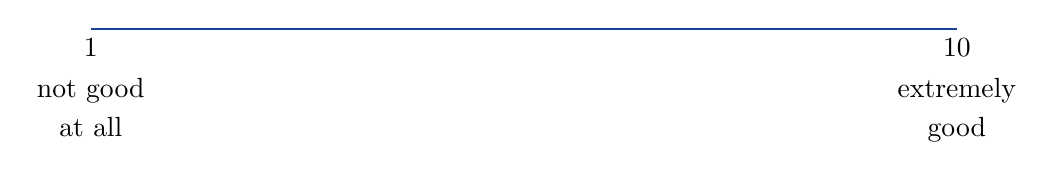
\begin{tikzpicture}
    % Draw the main line
    \draw[thick, WHUblue] (0,0) -- (10,0);
    \draw[thick, WHUblue] (0,0) -- (-1,0);

    % Add labels for the ends
    \node[below] at (-1,0) {1};
    \node[below] at (10,0) {10};

    % Add text for the left label
    \node[below] at (-1,-0.5) {not good};
    \node[below] at (-1,-1) {at all};

    % Add text for the right label
    \node[below] at (10,-0.5) {extremely};
    \node[below] at (10,-1) {good};
\end{tikzpicture}
\end{center}
\end{frame}


\begin{frame}\frametitle{How good do you consider yourself?}
\begin{center}
  
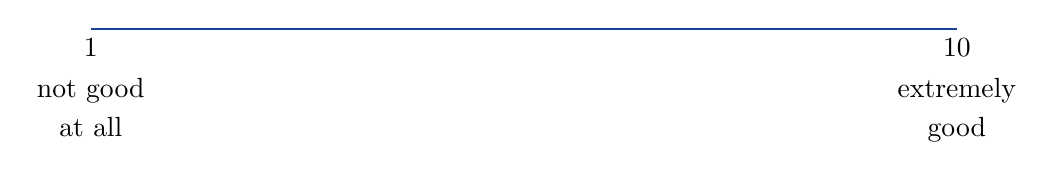
\begin{tikzpicture}
    % Draw the main line
    \draw[thick, WHUblue] (0,0) -- (10,0);
    \draw[thick, WHUblue] (0,0) -- (-1,0);

    % Add labels for the ends
    \node[below] at (-1,0) {1};
    \node[below] at (10,0) {10};

    % Add text for the left label
    \node[below] at (-1,-0.5) {not good};
    \node[below] at (-1,-1) {at all};

    % Add text for the right label
    \node[below] at (10,-0.5) {extremely};
    \node[below] at (10,-1) {good};
\end{tikzpicture}
\end{center}
\end{frame}

\twocolslide{“The Illusion of Moral Superiority”}{
\begin{itemize}
  \item Participants of an Experiment were asked to rate the judgements for the Self and the average person (Other) were provided on a scale from 1 (not at all) to 7 (very much so).
  \item The mean scores for Self are generally higher for positive traits and lower for negative traits when compared to ratings for Others, indicating a tendency for individuals to view themselves in a more favorable light. 
\end{itemize}
}
{\includegraphics[height=6.5cm]{pics/tappin.PNG}
\source{Tappin \& McKay (2017)}
}{0.495}{0.4}

\begin{frame}
\frametitle{What is Moral?}

  \begin{itemize}
    \item \textbf{Origin:} \textit{moralis} (Latin) — concerning custom; \textit{mos, mores} — custom(s)
    \item \textbf{Definition:} A system of norms that guide human behavior
    \item \textbf{Claim:} These norms have an \textcolor{WHUblue}{unconditional claim to validity}
  \end{itemize}

\vspace{0.5em}

\textbf{Moral Judgments:}
\begin{itemize}
  \item \textcolor{WHUblue}{\textbf{Moral}} = morally good
  \item \textcolor{WHUblue}{\textbf{Immoral}} = morally evil, wrong, bad
\end{itemize}

\vspace{0.5em}

\textbf{Types of Norms:}
\begin{itemize}
  \item \textbf{Moral norms}
  \item \textbf{Social norms}
  \item \textbf{Legal norms}
\end{itemize}

\source{Hübner (2014)}
\end{frame}

\begin{frame}
\frametitle{What is Ethics?}

\begin{center}
  \textcolor{WHUblue}{\Large\textbf{Ethics}}\\[0.5em]
  \textcolor{gray}{\textit{(from Greek: \textcolor{red}{character, disposition, habit, custom, convention})}}
\end{center}

\vspace{1em}

\begin{itemize}
  \item Ethics is the \textbf{science of morality}.
  \item \textit{Ethical} = belonging to the science of ethics
  \item \textit{Unethical} = contrary to ethical principles
\end{itemize}

\vspace{1em}

\textbf{Branches of Ethics:}
\begin{itemize}
  \item \textcolor{WHUblue}{\textbf{Descriptive Ethics}}: What moral systems exist? Under what conditions do people follow moral norms?
  \item \textcolor{WHUblue}{\textbf{Normative Ethics}}: How can moral systems be justified?
\end{itemize}

\vspace{1em}

\textbf{Application Areas:} \textcolor{gray}{bioethics, medical ethics, business ethics, and more}

\vspace{0.5em}
\hfill\source{Hübner (2014)}
\end{frame}

% Slide 4
\begin{frame}
\frametitle{Example: Descriptive Ethics}

\begin{tcolorbox}[colback=WHUblue!5!white, colframe=WHUblue, title=Adam Smith, fonttitle=\bfseries, sharp corners=south]
\textit{
"How selfish soever man may be supposed, there are evidently some principles in his nature, which interest him in the fortune of others, and render their happiness necessary to him, though he derives nothing from it except the pleasure of seeing it. Of this kind is \textbf{pity or compassion}, the emotion which we feel for the misery of others, when we either see it, or are made to conceive it in a very lively manner. That we often derive \textcolor{WHUblue}{sorrow from the sorrow of others}, is a matter of fact too obvious to require any instances to prove it; for this sentiment, like all the other original passions of human nature, is by no means confined to the virtuous and humane, though they perhaps may feel it with the most exquisite sensibility. \textcolor{WHUblue}{The greatest ruffian, the most hardened violator of the laws of society, is not altogether without it.}"
}
\end{tcolorbox}

\vspace{0.5em}
\hfill\scriptsize--- Adam Smith (1723--1790)
\end{frame}

\twocolslide{Normative Ethics: Teleology (telos) = end or purpose}{
  \begin{itemize}
      \item \textbf{Jeremy Bentham (1748–1832)}
      \item[] \textit{“Nature has placed mankind under the governance of two sovereign masters, pain and pleasure. It is for them alone to point out what we ought to do, as well as to determine what we shall do.”} \\
  \end{itemize}
  \source{An Introduction to the Principles of Morals and Legislation (1789)}
  
}{  \centering
    \includegraphics[width=0.5\linewidth]{pics/bentham.jpg} % Replace with actual image file if used
  }{0.6}{0.39}
  
\twocolslide{Normative Ethics: Teleology (telos) = end or purpose}{
      \begin{itemize}
      \item \textbf{John Stuart Mill (1806–1873)}
      \item[] \textit{“It is better to be a human being dissatisfied than a pig satisfied; better to be Socrates dissatisfied than a fool satisfied. And if the fool, or the pig, is of a different opinion, it is only because they know their own side of the question.”} \\
      \end{itemize}  
      \source{Utilitarianism (1863)}
}{ \centering
    \includegraphics[width=0.5\linewidth]{pics/mill.jpg} % Replace with actual image file if used
  }{0.6}{0.39}
  
\twocolslide{Title}{
here comes the textr
}
{\includegraphics[height=3cm]{pics/WHU_Logo_RGB_Screen.jpg}
}{0.4}{0.6}


\twocolslide{Normative Ethics: Deontology}{
  \begin{itemize}
    \item \textbf{Immanuel Kant (1724–1804)}
      \item[] \textit{“There is nothing in the world, indeed nothing even beyond it, that could be regarded as good without qualification — except \textcolor{WHUblue}{\textbf{a good will}}.”} \\
      \end{itemize}
      \source{Groundwork of the Metaphysics of Morals (1785)}
}{
  \includegraphics[height=4cm]{pics/kant.jpg}
}{.6}{.39}

\twocolslide{Normative Ethics: Deontology}{
  	\begin{itemize}
      \item \textbf{John Rawls (1921–2002)}
      \item[] \textit{“\textcolor{WHUblue}{Justice is the first virtue of social institutions}, as truth is of systems of thought. A theory however elegant and economical must be rejected or revised if it is untrue; likewise \textcolor{WHUblue}{laws and institutions no matter how efficient and well-arranged must be reformed or abolished if they are unjust}.”} \\
    \end{itemize}
    \source{A Theory of Justice (1971)}
}{
  \includegraphics[height=4cm]{pics/rawls.png}
}{.6}{.39}


\twocolslide{Normative Ethics: Virtue Ethics}{
 \begin{itemize}
      \item \textbf{Plato (428/427 BC – 348/347 BC)}
      \item[] Plato distinguishes three parts of the soul: reason, desire, and will (as the spirited part of the soul). He names four virtues:
      \begin{itemize}
        \item \textbf{Wisdom}: reason recognizes what is beneficial to the soul
        \item \textbf{Courage}: persistence in what reason deems right
        \item \textbf{Temperance}: harmony between the parts, acknowledging reason's rule
        \item \textbf{Justice}: each part of the soul does its own proper task
      \end{itemize}
    \end{itemize}
    \source{Politeia, 427a–434c}    
}{
  \includegraphics[width=0.7\linewidth]{pics/plato.jpg} 
}{0.7}{.29}

\twocolslide{Normative Ethics: Virtue Ethics}{
  \begin{itemize}
      \item \textbf{Aristotle (384 BC – 322 BC)}
      \item[] 
      \textit{“\textcolor{WHUblue}{Virtue}, then, is a \textcolor{WHUblue}{state of character} concerned with \textcolor{WHUblue}{choice}, lying in a \textcolor{WHUblue}{mean}, i.e. the mean relative to us, this being determined by \textcolor{WHUblue}{reason} and by that reason by which the man of \textcolor{WHUblue}{practical wisdom} would determine it. And it is a mean between two \textcolor{WHUblue}{vices}, that which depends on \textcolor{WHUblue}{excess} and that which depends on \textcolor{WHUblue}{defect}.”}
    \end{itemize}
    \source{Nicomachean Ethics II.6}    
}{
  \centering \includegraphics[width=0.5\linewidth]{pics/aris.jpg} 
}{0.65}{.34}

\begin{frame}
\frametitle{What is “business ethics”? What is “behavioral ethics”?}

\begin{columns}[T,onlytextwidth]
  \begin{column}{0.48\textwidth}
    \textcolor{WHUblue}{\Large\textbf{Business Ethics}}
    \vspace{0.5em}
    \begin{itemize}
      \item Principles and reasons that \textbf{should} guide conduct in business
      \item How to put moral norms \textbf{into practice} in organizations and markets
      \item Focus on \textbf{moral standards} applied by individuals in business contexts
    \end{itemize}
  \end{column}
  \begin{column}{0.04\textwidth}
    \centering
    \vspace{2em}
    \textcolor{gray}{\Large\textbf{\&}}
  \end{column}
  \begin{column}{0.48\textwidth}
    \textcolor{WHUblue}{\Large\textbf{Behavioral Ethics}}
    \vspace{0.5em}
    \begin{itemize}
      \item Studies how people \textbf{actually behave} in ethical dilemmas
      \item Explores why actions may differ from moral ideals
      \item Examines behavior judged by generally accepted norms
    \end{itemize}
  \end{column}
\end{columns}

\vspace{1em}
\centering
\textcolor{gray}{\footnotesize\textit{Behavioral ethics is a subfield of business ethics that investigates how people actually behave in ethical situations, complementing the normative question of what they should do.}}
\end{frame}

\begin{frame}{Sustainable Development}

\begin{tcolorbox}[colback=WHUblue!5!white, colframe=WHUblue, title=Definition, fonttitle=\bfseries, sharp corners=south]
Sustainable development is development that meets the needs of the present without compromising the ability of future generations to meet their own needs.
\end{tcolorbox}

\vspace{1em}

\textbf{Key Principles:}
\begin{itemize}
  \item Intergenerational equity: Balancing current and future needs.
  \item Integration of economic, environmental, and social considerations.
  \item Long-term planning and responsible resource management.
\end{itemize}

\vspace{1em}

\textbf{Application in Business:}
\begin{itemize}
  \item Implementing sustainable supply chain practices.
  \item Investing in renewable energy and reducing carbon footprint.
  \item Engaging in corporate social responsibility initiatives.
\end{itemize}
\source{Brundtland Report, 1987}
\end{frame}

\begin{frame}{Stakeholder Theory}

\begin{tcolorbox}[colback=WHUblue!5!white, colframe=WHUblue, title=Definition, fonttitle=\bfseries, sharp corners=south]
Stakeholder theory posits that businesses should create value for all stakeholders—not just shareholders—including employees, customers, suppliers, communities, and financiers.
\end{tcolorbox}

\vspace{1em}

\textbf{Key Points:}
\begin{itemize}
  \item Emphasizes ethical obligations to all parties affected by business operations.
  \item Encourages long-term value creation and trust-building.
  \item Forms the ethical foundation for ESG and CSR initiatives.
\end{itemize}

\vspace{1em}

\textbf{Example:} \\
A company implementing sustainable practices to benefit both the environment and local communities, not solely focusing on profit maximization.

\source{Freeman, 1984; Darden School of Business, 2024}
\end{frame}

\begin{frame}{Compliance}

\begin{tcolorbox}[colback=WHUblue!5!white, colframe=WHUblue, title=Definition, fonttitle=\bfseries, sharp corners=south]
Compliance involves adhering to laws, regulations, standards, and ethical practices relevant to an organization's operations.
\end{tcolorbox}

\vspace{1em}

\textbf{Key Components:}
\begin{itemize}
  \item Legal compliance: Following applicable laws and regulations.
  \item Ethical compliance: Upholding internal codes of conduct and ethical standards.
  \item Risk management: Identifying and mitigating compliance risks.
\end{itemize}

\vspace{1em}

\textbf{Importance:}
\begin{itemize}
  \item Prevents legal penalties and reputational damage.
  \item Enhances organizational integrity and stakeholder trust.
  \item Supports sustainable and ethical business practices.
\end{itemize}
\source{EQS Group, 2024}

\end{frame}

\begin{frame}[t]{Corporate Social Responsibility (CSR)}

\begin{tcolorbox}[colback=WHUblue!5!white, colframe=WHUblue, title=Definition, fonttitle=\bfseries, sharp corners=south]
CSR refers to a company's \textbf{voluntary commitment} to integrate social and environmental concerns into its business operations and stakeholder interactions—going beyond legal compliance.
\end{tcolorbox}

\vspace{0.8em}

\begin{columns}[T,onlytextwidth]
  \begin{column}{0.48\textwidth}
    \textcolor{WHUblue}{\textbf{Key Characteristics}}
    \begin{itemize}
      \item Voluntary and values-driven
      \item Focus on stakeholder expectations
      \item Long-term trust-building
      \item Initiatives: sustainability, community, fair employment
    \end{itemize}
  \end{column}
  \begin{column}{0.04\textwidth}
    \hfill
  \end{column}
  \begin{column}{0.48\textwidth}
    \textcolor{WHUblue}{\textbf{Relation to ESG}}
    \begin{itemize}
      \item \textbf{ESG:} Measurable criteria for investors
      \item \textbf{CSR:} Internal ethical stance and practical initiatives
      \item CSR often fulfills or anticipates ESG expectations
    \end{itemize}
  \end{column}
\end{columns}

\vspace{0.8em}

%\begin{block}{\textbf{Example}}
%A firm voluntarily offsetting carbon emissions, publishing a social impact report, or partnering with NGOs—even in the absence of regulatory pressure.
%\end{block}

%\vspace{0.2em}
\hfill\source{European Commission, 2011}
\end{frame}

\begin{frame}{ESG: Environmental, Social, Governance}

\begin{tcolorbox}[colback=WHUblue!5!white, colframe=WHUblue, title=Definition, fonttitle=\bfseries, sharp corners=south]
ESG stands for \textbf{Environmental, Social, and Governance}—three key dimensions for evaluating a company’s sustainability, ethical impact, and responsible management. ESG criteria are used by investors, regulators, and stakeholders to assess long-term value and risk.
\end{tcolorbox}
\vspace{1em}
\begin{columns}[T,onlytextwidth]
  \begin{column}{0.33\textwidth}
    \textcolor{WHUblue}{\textbf{Environmental}}
    \begin{itemize}
      \item Climate change mitigation and adaptation
      \item Energy efficiency and renewable energy use
      \item Resource conservation (water, raw materials)
      %\item Pollution and waste management
      %\item Biodiversity and ecosystem protection
    \end{itemize}
  \end{column}
  \begin{column}{0.33\textwidth}
    \textcolor{WHUblue}{\textbf{Social}}
    \begin{itemize}
      \item Employee well-being, health, and safety
      %\item Diversity, equity, and inclusion (DEI)
      \item Human rights and labor standards
      %\item Community engagement and social impact
      \item Customer protection and product responsibility
    \end{itemize}
  \end{column}
  \begin{column}{0.33\textwidth}
    \textcolor{WHUblue}{\textbf{Governance}}
    \begin{itemize}
      \item Board structure and diversity
      \item Anti-corruption
      \item Executive compensation alignment
      \item Transparency and reporting
      %\item Risk management and compliance
    \end{itemize}
  \end{column}
\end{columns}
\source{OECD, 2025}
\end{frame}

\begin{frame}{ESG: Environmental, Social, Governance}
\textbf{Why ESG Matters:}
\begin{itemize}
  \item \textbf{Investment:} ESG criteria guide investors toward sustainable, ethical companies with better long-term prospects.
  \item \textbf{Risk:} Strong ESG practices help firms manage environmental, social, and governance risks.
  \item \textbf{Compliance:} ESG reporting standards (e.g., EU Sustainable Finance Disclosure Regulation) require disclosure, affecting reputation and legal standing.
\end{itemize}

\vspace{0.5em}

\textbf{Current Trends:}
\begin{itemize}
  \item ESG investing is gaining momentum, with significant growth in ESG-focused funds globally.
  \item Companies are integrating ESG considerations into their core strategies to meet stakeholder expectations and regulatory requirements.
\end{itemize}
\end{frame}

\begin{frame}
\frametitle{\textbf{Descriptive and Normative Ethics}}

\begin{itemize}
  \item \textcolor{WHUblue}{\textbf{Elements of descriptive ethics:}}
  \begin{itemize}
    \item Collecting information on business values
    \item Analyzing the belief structure of a particular corporate culture
    \item Data analysis of the actual decision-making habits
    \item Analysis of case studies on decision-making habits
  \end{itemize}

  \vspace{0.5em}

  \item \textcolor{WHUblue}{\textbf{Elements of normative ethics:}}
  \begin{itemize}
    \item Study and development of moral standards, rules, and procedures
    \item Study of the viability of these, i.e., the possibility of their practical application in particular contexts
  \end{itemize}

  \vspace{0.5em}

  \item \textcolor{WHUblue}{\textbf{The distinction between the two allows to distinguish between:}}
  \begin{itemize}
    \item What is accepted practice in a particular set of situations/contexts
    \item What a particular institution or culture holds to be acceptable/valuable
  \end{itemize}
\end{itemize}

\end{frame}

\begin{frame}{Four Layers of Business and Economic Ethics}

\begin{columns}[T,onlytextwidth]
  \begin{column}{0.48\textwidth}
    \textcolor{WHUblue}{\textbf{Supralevel:}} International level (international business \& economic ethics)
    \begin{itemize}
      \item \textit{If governments are involved in the economy, how should nation-states interact?}
    \end{itemize}
    \vspace{1em}
    \textcolor{WHUblue}{\textbf{Mesolevel:}} Institutional / company level (business ethics)
    \begin{itemize}
      \item \textit{Can a corporation bear responsibility for its actions? Can companies act?}
      \item \textit{How can a company ensure its ethical behavior?}
    \end{itemize}
  \end{column}
  \begin{column}{0.48\textwidth}
    \textcolor{WHUblue}{\textbf{Macrolevel:}} Societal level (economic ethics)
    \begin{itemize}
      \item \textit{Should the government be involved in the economic cycle? If yes, what kind of regulation does the economy need?}
    \end{itemize}
    \vspace{2em}
    \textcolor{WHUblue}{\textbf{Microlevel:}} Individual level (behavioral ethics)
    \begin{itemize}
      \item \textit{(How) can employees bear responsibilities for their actions? Can they act ethically?}
    \end{itemize}
  \end{column}
\end{columns}

\end{frame}

% Slide 1: The Dieselgate Scandal
\begin{frame}
\frametitle{Dieselgate: A Case for Business Ethics}

\begin{tcolorbox}[colback=WHUblue!5!white, colframe=WHUblue, title=The Dieselgate Scandal, fonttitle=\bfseries, sharp corners=south]
\textbf{Volkswagen (VW) installed software in millions of diesel vehicles to cheat emissions tests, allowing cars to pass regulatory standards while emitting pollutants far above legal limits during real-world driving.}
\end{tcolorbox}

\vspace{1em}

\textbf{Why is Dieselgate a Tension Point for Business Ethics?}
\begin{itemize}
  \item \textbf{Profit vs. Principle:} Volkswagen chose to increase sales and profits by cheating emissions tests, instead of following legal and ethical standards.
  \item \textbf{Short-term Gain, Long-term Risk:} The company’s decision to deceive regulators and consumers brought immediate financial benefits, but ultimately resulted in billions in fines, criminal charges, and lasting reputational harm.
  \item \textbf{Systemic Issues:} The scandal was not just the result of a few bad actors—it reflected deeper problems in VW’s corporate culture, incentive structures, and industry-wide pressures that encouraged unethical behavior.
\end{itemize}

\vspace{0.5em}
\begin{center}
%\includegraphics[height=2.5cm]{pics/dieselgate.jpg}
\end{center}

\source{Based on EPA, 2015; The Guardian, 2017}
\end{frame}

% Slide 2: Pro-Social Motivation and Stakeholder Impact
\begin{frame}
\frametitle{Dieselgate: Pro-Social Motivation and Stakeholder Impact}

\begin{tcolorbox}[colback=WHUblue!5!white, colframe=WHUblue, title=Environmental Goals and Ethical Tensions, fonttitle=\bfseries, sharp corners=south]
\textbf{VW's stated aim was to develop "clean diesel" vehicles—combining performance, efficiency, and lower emissions to meet environmental goals and appeal to eco-conscious consumers.}
\end{tcolorbox}

\vspace{1em}

\textbf{Ethical Tensions and Stakeholder Impact:}
\begin{itemize}
  \item \textbf{Pro-Social Motivation:} Volkswagen publicly promoted its commitment to environmental protection and innovation by developing “clean diesel” vehicles.
  \item \textbf{Unethical Means to Noble Ends:} Although the company aimed to achieve environmental goals, it used deceptive software to cheat emissions tests, violating ethical and legal standards.
  \item \textbf{Negative Stakeholder Impact:} The deception harmed multiple stakeholders—including customers (misled about emissions), regulators (undermined trust), the environment (increased pollution), and public health (higher exposure to pollutants).
  \item \textbf{Ethical Lesson:} Positive intentions or goals do not excuse unethical actions; both the means and the ends must be ethically sound.
\end{itemize}

\source{Based on EPA, 2015; The Guardian, 2017}
\end{frame}


% Slide 1: The Problem and the Shift to Shared Value
\begin{frame}[t]
\frametitle{\textbf{Michael Porter: Creating Shared Value}}

\begin{tcolorbox}[colback=WHUblue!5!white, colframe=WHUblue, title=The Traditional View, fonttitle=\bfseries, sharp corners=south]
“In neoclassical thinking, a requirement for social improvement [...] imposes a constraint on the corporation. Adding a constraint to the firm that is already maximizing profits, says the theory, will inevitably raise costs and reduce profits.”

\vspace{0.5em}

Corporate responsibility programs—reaction to external pressure—have emerged largely to improve firms’ reputations and are treated as a necessary expense. Anything more is seen by many as an irresponsible use of shareholders’ money.
\end{tcolorbox}

\vspace{1em}

  \source{Michael Porter, \textit{Harvard Business Review} (2011)}
\end{frame}

% Slide 2: The Shared Value Concept
\begin{frame}[t]
\frametitle{\textbf{Michael Porter: Creating Shared Value}}

\begin{tcolorbox}[colback=WHUblue!5!white, colframe=WHUblue, title=The Shared Value Approach, fonttitle=\bfseries, sharp corners=south]
\textcolor{WHUblue}{\textbf{“The concept of shared value, in contrast, recognizes that societal needs, not just conventional economic needs, define markets. It also recognizes that social harms or weaknesses frequently create internal costs for firms.”}}

\vspace{0.7em}

...companies have overlooked opportunities to meet fundamental societal needs and misunderstood how societal harms and weaknesses affect value chains. Our field of vision has simply been too narrow.

\vspace{0.7em}

\textcolor{WHUblue}{\textbf{“Companies can create economic value by creating societal value. There are three distinct ways to do this: by reconceiving products and markets, redefining productivity in the value chain, and building supportive industry clusters at the company’s locations.”}}
\end{tcolorbox}

\vspace{1em}

  \source{Michael Porter, \textit{Harvard Business Review} (2011)}
\end{frame}


\subsection{Procedural Details}
\twocolslide{About me}{

\textbf{Education}
\begin{itemize}
  \item University Bonn (Dipl.)
  \item University of Cologne (PhD)
  \item Joined WHU in 2016
  \item Full Professor of Behavioral Economics since 2025
\end{itemize}
\textbf{Teaching Experience}
\begin{itemize}
  \item Bachelor, Master, and MBA level
\end{itemize}

\textbf{Research Interest}
\begin{itemize}
  \item Behavioral and Experimental Economics
  \item Interaction of Humans and Machines (AI)
  \item Incentives and Ethical Behavior
\end{itemize}

}{
\centering
\includegraphics[height=6cm]{pics/rilke.PNG}
}{0.6}{0.4}

\begin{frame}
\frametitle{Course Schedule}
\centering
\begin{tabular}{@{}lcp{8cm}@{}}
\toprule
\textbf{Date} & \textbf{Session} & \textbf{Topic} \\
\midrule
Sep 5   & 1 & Introduction to Business Ethics \\
Sep 12  & 2 & Ethical Theories and Frameworks \\
Sep 19  & 3 & Behavioral Ethics: Why Good People Do Bad Things \\
Sep 26  & 4 & Ethics in Corporate Decision-Making \\
Oct 3   & 5 & Fairness, Justice, and Moral Intuition \\
Oct 10  & 6 & Case Study Discussion and Wrap-Up \\
\midrule
Oct 17  & &\textbf{Final Exam} \\
\bottomrule
\end{tabular}
\end{frame}

\begin{frame}{Lecture Materials}

\begin{itemize}
  \item All materials (slides, readings, cases, and additional resources) are available on the course GitHub repository:
  
  \vspace{0.5em}
  \begin{center}
      \texttt{\href{https://github.com/rrilke/BusinessEthics-WHU}{github.com/rrilke/BusinessEthics-WHU}}
  \end{center}
  \vspace{0.5em}

  \item Please check the repository regularly — it is the central source for everything.
  
  \item \textbf{Readings are essential:}
  \begin{itemize}
    \item \textbf{Required readings} must be read \emph{before class}.
    \item They are fundamental to understanding the course content and performing well in the final exam.
  \end{itemize}
  \item \textbf{Optional readings} are for those who want to dig deeper — or outperform everyone else. 
  \item I expect thoughtful and active engagement with the texts. They are not decorative.
\end{itemize}

\end{frame}
 
\begin{frame}
\frametitle{Final Exam}

\begin{itemize}
  \item \textbf{Duration:} 90 minutes
  \item \textbf{Total points:} 100
  \item \textbf{Format:}
  \begin{itemize}
    \item Multiple-choice questions
    \item Case study-based analysis
    \item Open-ended questions on key concepts discussed in class
  \end{itemize}
  \item \textbf{Scope:} All lecture content and required readings
  \item \textbf{Grading:} According to the official WHU grading scale
  \item \textbf{Focus:} Apply what you’ve learned — not just reproduce it
  \begin{itemize}
    \item You will be asked to transfer concepts to unfamiliar, real-world scenarios
  \end{itemize}
\end{itemize}

\vspace{0.8em}
\centering
\textit{Tip: Understanding and flexible thinking matter more than memorization.}
\end{frame}

\begin{frame}
\frametitle{ChatGPT Exam Question Challenge}

\begin{itemize}
  \item \textbf{Optional bonus assignment:} earn up to \textbf{10 extra points}
  \item Submit \textbf{5 self-generated exam-style questions} created using ChatGPT
  \begin{itemize}
    \item Varying difficulty: at least one basic, others more advanced
    \item Include different course topics and formats (MC or open-ended)
    \item Each question must include a \textbf{model answer}
  \end{itemize}
  \item Submit detailed documentation for each question:
  \begin{itemize}
    \item Prompt(s) used with ChatGPT
    \item ChatGPT’s raw output
    \item Short reflection on the process (2–4 sentences)
  \end{itemize}
  \item \textbf{Format:} PDF or Markdown file, named \texttt{Lastname\_Firstname\_BonusQuestions.pdf}
  \item \textbf{Deadline:} \textit{[Insert Date]}
\end{itemize}

\vspace{0.8em}
\centering
\textit{A chance to deepen your understanding and critically explore generative AI in learning.}
\end{frame}



\end{document}